\documentclass[11pt,a4paper]{article}

\usepackage[a4paper,top=1in,bottom=1in,left=1.1in,right=1.1in]{geometry}
\usepackage[T1]{fontenc}
\usepackage[utf8]{inputenc}
\usepackage{mathptmx}
\usepackage{titlesec}
\usepackage{fancyhdr}
\usepackage{enumitem}
\usepackage{array}
\usepackage{tabularx}
\usepackage{booktabs}
\usepackage{longtable}
\usepackage{tikz}
\usetikzlibrary{arrows.meta,positioning}
\usepackage{caption}
\usepackage{setspace}
\usepackage[hidelinks]{hyperref}

\titleformat{\section}
  {\normalfont\Large\bfseries}
  {\thesection}{0.6em}{}
\titleformat{\subsection}
  {\normalfont\large\bfseries}
  {\thesubsection}{0.6em}{}
\titleformat{\subsubsection}
  {\normalfont\normalsize\bfseries\itshape}
  {\thesubsubsection}{0.6em}{}

\titlespacing*{\section}{0pt}{16pt}{8pt}
\titlespacing*{\subsection}{0pt}{10pt}{5pt}

\pagestyle{fancy}
\fancyhf{}
\renewcommand{\headrulewidth}{0.4pt}
\renewcommand{\footrulewidth}{0.4pt}
\fancyhead[L]{\small NimbusVault -- Project Proposal}
\fancyhead[R]{\small UCS503P}
\fancyfoot[L]{\small Thapar Institute of Engineering and Technology}
\fancyfoot[R]{\small \thepage}

\fancypagestyle{plain}{
  \fancyhf{}
  \renewcommand{\headrulewidth}{0pt}
  \fancyfoot[C]{\small\thepage}
}

\setlength{\parindent}{0pt}
\setlength{\parskip}{6pt}
\onehalfspacing
\renewcommand{\arraystretch}{1.25}

\begin{document}

\begin{titlepage}
\centering
\thispagestyle{empty}

\vspace*{0.8cm}
\rule{\linewidth}{0.8pt}

\vspace{0.5cm}
{\Large \textbf{THAPAR INSTITUTE OF ENGINEERING AND TECHNOLOGY}}\\[4pt]
{\large (Deemed to be University), Patiala}\\[10pt]
{\large\textbf{Department of Computer Science and Engineering}}

\vspace{0.5cm}
\rule{\linewidth}{0.8pt}

\vspace{2.4cm}

{\large\bfseries A Project Proposal Report}\\[6pt]
{\normalsize on}\\[10pt]

{\huge \textbf{NimbusVault}}\\[8pt]
{\Large AI-Powered Cloud Storage \& Document Intelligence Platform}

\vspace{1.8cm}

\begin{tabular}{ll}
\textbf{Course:} & UCS503P -- Project Proposal \\[4pt]
\textbf{Academic Year:} & 2028 \\[4pt]
\textbf{Programme:} & B.E./B.Tech. Computer Engineering, 3\textsuperscript{rd} Year \\
\end{tabular}

\vspace{2.2cm}

\begin{minipage}{0.46\textwidth}
\centering
\textbf{Submitted By} \\[10pt]
\begin{tabular}{@{}ll@{}}
\textbf{Name} & \textbf{Roll No.} \\
\midrule
Mehul Jain & 1024030020 \\
Saras & 1024030021 \\
Mansimar & 1024030012 \\
\end{tabular}
\end{minipage}%
\begin{minipage}{0.46\textwidth}
\centering
\textbf{Submitted To} \\[10pt]
Paramveer Sidhu \\
Department of Computer Science \\ and Engineering \\
Thapar Institute of Engineering \\ and Technology
\end{minipage}

\vfill

\rule{\linewidth}{0.5pt}\\[4pt]
{\normalsize \today}\\[4pt]
\rule{\linewidth}{0.5pt}

\end{titlepage}


\pagestyle{plain}
\tableofcontents
\newpage
\pagestyle{fancy}
\setcounter{page}{1}


\section*{Abstract}
\addcontentsline{toc}{section}{Abstract}

NimbusVault is a cloud-based file storage and document intelligence platform developed to address the limitations of conventional local and legacy cloud storage systems. The design draws on established cloud storage architectures such as Google Drive and Dropbox, combining scalable object storage with a document understanding layer to provide secure file management along with intelligent search.

The system separates file storage from file metadata. Raw files are stored on Amazon S3, while metadata such as ownership, folder structure, permissions and file attributes is stored in a PostgreSQL database accessed through the Prisma ORM. File transfers use pre-signed URLs, so uploads and downloads happen directly between the browser and S3 without passing through the backend server. This keeps load off the backend and allows files of any size to be handled efficiently.

In addition to standard storage operations such as upload, download, folder organisation and file sharing, NimbusVault includes an AI-based document intelligence feature built around a Retrieval-Augmented Generation (RAG) pipeline. Uploaded documents are parsed, split into chunks and converted into vector embeddings, which are stored in a vector database. This lets users search their documents by meaning rather than by exact keywords, and ask questions about document content in natural language.

The platform uses JWT-based authentication, password hashing, AWS IAM policies and role-based access control to protect user data and shared resources. The backend is stateless and can run across multiple instances, so the system can scale horizontally as usage increases. Taken together, the project combines full-stack development, cloud infrastructure and applied AI in one system, and is intended to demonstrate practical engineering ability across each of these areas.

\newpage

\section{Introduction}

The amount of digital data generated by individuals and organisations has grown rapidly over the last decade, driven by high-resolution media, collaborative documents, and everyday digital records. This growth has exposed several limitations of traditional file storage, which was not built to handle data at this scale or to support the kind of remote, always-available access that most users now expect.

Storing files only on local devices, such as hard drives, USB drives or unmanaged network shares, comes with well-known problems. Storage capacity is limited, hardware can fail, and files kept on one device are not accessible from another. A single disk failure can mean permanent data loss. These limitations are part of why cloud storage has become the standard approach for personal and organisational data alike, since it removes the dependency on a single physical device and instead relies on distributed, redundant infrastructure.

Moving files to the cloud, however, does not solve every problem. As a user's collection of files grows, it becomes harder to locate a specific document through folder browsing or keyword search alone. Traditional storage systems understand file names, not the content of the files themselves, so users are left to remember roughly where or under what name something was saved.

Sharing is another area where common storage tools fall short. Users often need to share specific files with specific people for a limited period of time, without exposing their entire account, and this requires access-control features that many systems either do not offer or implement poorly.

NimbusVault is motivated by these three issues: the need for reliable, scalable cloud storage; the need for controlled and secure file sharing; and the need for search that understands document content rather than only file names. The project combines a conventional cloud storage architecture with an AI-based document intelligence layer, with the aim of showing how cloud infrastructure and applied AI can be combined within a single, practical system.

\section{Problem Statement}

The following problems are commonly observed in the way individuals and small teams store and manage files, even when cloud storage is already in use.

\begin{itemize}[leftmargin=1.2cm, itemsep=5pt]
    \item Personal devices have limited storage capacity, and users are often forced to delete or move files simply to free up space.
    \item Files kept only on local devices are vulnerable to hardware failure, theft and accidental deletion, with no built-in redundancy.
    \item As the number of stored files grows, manually maintained folder structures become inconsistent and difficult to navigate.
    \item Keyword-based search only matches file names or indexed terms, so it performs poorly when a user cannot recall the exact name of a file.
    \item Existing storage systems have no understanding of what a document actually contains, so summarising or answering questions about a file requires opening and reading it manually.
    \item Sharing files securely is difficult: many tools either grant broad access to an entire account or rely on informal methods such as emailing attachments, with little control over expiry or permission level.
\end{itemize}

These issues together point to the need for a storage platform that is not only reliable and secure, but also able to understand the content it stores.


\section{Project Objectives}

\begin{enumerate}[leftmargin=1.2cm, itemsep=5pt]
    \item Build a cloud-native storage platform that can handle files at scale with high availability.
    \item Implement secure user authentication using standard protocols and password-handling practices.
    \item Use AWS S3 for scalable, durable object storage of user files.
    \item Keep file metadata (in PostgreSQL) separate from raw file objects (in AWS S3), so each layer can be scaled independently.
    \item Implement pre-signed URL based file transfer, allowing uploads and downloads to go directly between the browser and S3.
    \item Provide secure, permission-based file sharing with configurable access levels and link expiry.
    \item Integrate an AI document assistant capable of semantic search and natural-language question answering over stored documents.
\end{enumerate}

\section{Proposed Solution}

NimbusVault addresses the problems described above through a full-stack cloud storage platform, organised into core storage features, sharing and access-control features, and an AI document intelligence layer.

\subsection{Core Features}
\begin{itemize}[leftmargin=1.2cm, itemsep=3pt]
    \item User registration and login with JWT-based authentication
    \item File upload and download via pre-signed AWS S3 URLs
    \item Folder creation and management
    \item Search and filtering across files and folders
    \item In-browser preview for common file types
    \item Trash and restore for deleted files
    \item Storage analytics showing usage by file type, folder and time
\end{itemize}

\subsection{Sharing and Access Control}
\begin{itemize}[leftmargin=1.2cm, itemsep=3pt]
    \item Shareable links with configurable permissions
    \item Expiring access for time-bound sharing
    \item Role-based access (owner, editor, viewer)
    \item File versioning to preserve and restore earlier versions
\end{itemize}

\subsection{AI Document Intelligence}
\begin{itemize}[leftmargin=1.2cm, itemsep=3pt]
    \item Automated text extraction from uploaded documents
    \item Semantic search based on document meaning, not just keywords
    \item Natural-language question answering over document content
    \item A Retrieval-Augmented Generation (RAG) pipeline that grounds AI answers in the user's own files
\end{itemize}

\section{System Architecture}

NimbusVault follows a layered architecture that separates the frontend, application backend, metadata storage, file storage and AI processing into distinct components. Figure~\ref{fig:architecture} shows the overall flow of data between these layers.

\begin{figure}[h!]
\centering
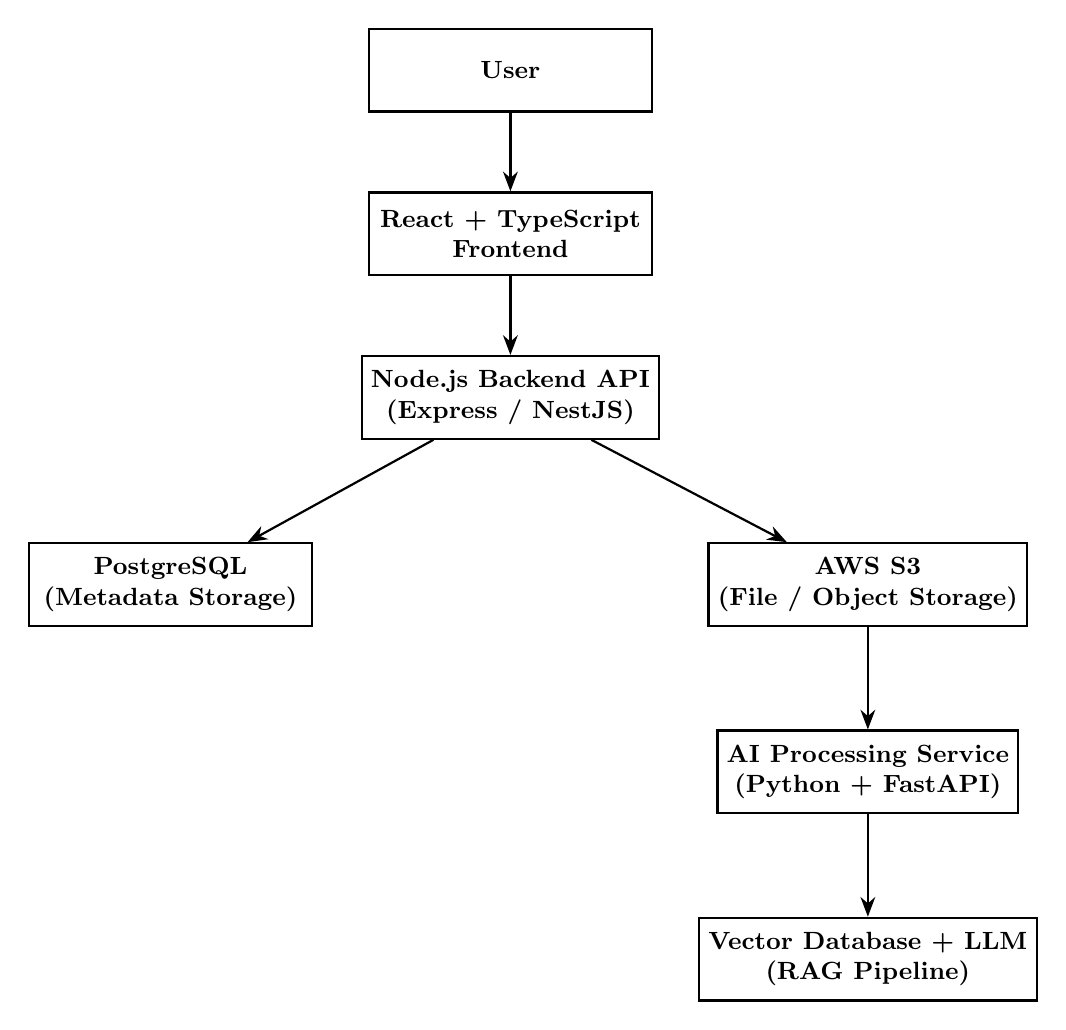
\begin{tikzpicture}[
    node distance=10mm and 14mm,
    box/.style={rectangle, draw=black, thick,
                minimum width=3.6cm, minimum height=1.05cm,
                align=center, font=\small\bfseries},
    arr/.style={-{Stealth[length=2.5mm]}, thick, draw=black}
]
    \node[box] (user) {User};
    \node[box, below=of user] (frontend) {React + TypeScript\\Frontend};
    \node[box, below=of frontend] (backend) {Node.js Backend API\\(Express / NestJS)};

    \node[box, below left=13mm and 6mm of backend] (db) {PostgreSQL\\(Metadata Storage)};
    \node[box, below right=13mm and 6mm of backend] (s3) {AWS S3\\(File / Object Storage)};

    \node[box, below=13mm of s3] (ai) {AI Processing Service\\(Python + FastAPI)};
    \node[box, below=13mm of ai] (vecdb) {Vector Database + LLM\\(RAG Pipeline)};

    \draw[arr] (user) -- (frontend);
    \draw[arr] (frontend) -- (backend);
    \draw[arr] (backend) -- (db);
    \draw[arr] (backend) -- (s3);
    \draw[arr] (s3) -- (ai);
    \draw[arr] (ai) -- (vecdb);
\end{tikzpicture}
\caption{High-level system architecture of NimbusVault}
\label{fig:architecture}
\end{figure}

\subsection{Component Responsibilities}

The frontend, built with React, TypeScript and Tailwind CSS, is responsible for rendering the interface, managing client-side state, and making authenticated API requests. It also handles file transfer directly to and from AWS S3 using pre-signed URLs issued by the backend, rather than routing file data through the backend server.

The backend, built with Node.js and Express or NestJS, exposes REST APIs for authentication, file and folder management, sharing, and search. It is responsible for generating pre-signed S3 URLs, enforcing authorisation rules, and coordinating requests to the AI processing service.

The database layer uses PostgreSQL with the Prisma ORM to store structured metadata, including users, folders, files, share links and permissions. Using an ORM keeps database access type-safe and easier to maintain as the schema evolves.

AWS S3 provides durable, scalable storage for the actual file content. It is kept fully separate from the metadata layer, with access controlled through AWS IAM policies and time-limited pre-signed URLs.

The AI service, written in Python using FastAPI, performs text extraction, chunking and embedding generation for uploaded documents, and handles semantic search and question-answering requests by querying the vector database and coordinating with the language model.

\section{Core Workflow}

The end-to-end workflow of NimbusVault, from account creation to secure file access, proceeds as follows:

\begin{enumerate}[leftmargin=1.2cm, itemsep=4pt]
    \item A new user registers by providing basic credentials, which are validated and stored securely.
    \item The user logs in; on success, the backend issues a signed JWT access token.
    \item The user creates one or more folders to organise their files.
    \item The user selects a local file to upload to a given folder.
    \item The frontend requests a pre-signed upload URL from the backend.
    \item The backend validates the request, checks authorisation, and generates a time-limited pre-signed S3 URL.
    \item The frontend uploads the file directly to AWS S3 using that URL, without routing it through the backend.
    \item Once the upload succeeds, the backend stores the file's metadata (name, size, type, S3 key, owner, folder) in PostgreSQL.
    \item The file is now available for search, preview and download.
    \item The owner may generate a secure sharing link with a chosen permission level and expiry.
    \item When the shared link is accessed, the backend checks permissions and expiry before granting access to the file.
\end{enumerate}

\section{Technology Stack}

Table~\ref{tab:techstack} summarises the technologies proposed for each layer of NimbusVault.

\begin{longtable}{@{}>{\bfseries}p{3.4cm} p{10.6cm}@{}}
\caption{Proposed technology stack for NimbusVault} \label{tab:techstack} \\
\toprule
\textbf{Layer} & \textbf{Technologies} \\
\midrule
\endfirsthead
\toprule
\textbf{Layer} & \textbf{Technologies} \\
\midrule
\endhead
Frontend & React.js, TypeScript, Tailwind CSS, React Router, React Query \\
\midrule
Backend & Node.js, Express.js / NestJS, REST APIs, JWT, bcrypt \\
\midrule
Database & PostgreSQL, Prisma ORM \\
\midrule
Cloud & AWS S3, AWS EC2, AWS IAM, AWS CloudFront \\
\midrule
DevOps & Docker, Docker Compose, GitHub Actions, CI/CD \\
\midrule
AI / ML & Python, FastAPI, NLP, Embedding Models, Vector Database, RAG Pipeline, LLM Integration \\
\bottomrule
\end{longtable}
\section{Database Design}

The metadata layer of NimbusVault is organised around four core entities, described in Tables~\ref{tab:user} through~\ref{tab:sharelink}.

\begin{table}[h!]
\centering
\begin{tabular}{@{}p{3.2cm}p{9.6cm}@{}}
\toprule
\textbf{Field} & \textbf{Description} \\
\midrule
\texttt{id} & Unique identifier for the user \\
\texttt{name} & Display name of the user \\
\texttt{email} & Unique email address used for login \\
\texttt{passwordHash} & Salted hash of the user's password \\
\bottomrule
\end{tabular}
\caption{\texttt{User} entity}
\label{tab:user}
\end{table}

\begin{table}[h!]
\centering
\begin{tabular}{@{}p{3.2cm}p{9.6cm}@{}}
\toprule
\textbf{Field} & \textbf{Description} \\
\midrule
\texttt{id} & Unique identifier for the file \\
\texttt{filename} & Original name of the uploaded file \\
\texttt{ownerId} & Foreign key referencing the owning \texttt{User} \\
\texttt{folderId} & Foreign key referencing the parent \texttt{Folder} \\
\texttt{s3Key} & Object key locating the file within AWS S3 \\
\texttt{size} & File size in bytes \\
\texttt{mimeType} & MIME type of the stored file \\
\bottomrule
\end{tabular}
\caption{\texttt{File} entity}
\label{tab:file}
\end{table}

\begin{table}[h!]
\centering
\begin{tabular}{@{}p{3.2cm}p{9.6cm}@{}}
\toprule
\textbf{Field} & \textbf{Description} \\
\midrule
\texttt{id} & Unique identifier for the folder \\
\texttt{name} & Display name of the folder \\
\texttt{ownerId} & Foreign key referencing the owning \texttt{User} \\
\texttt{parentFolderId} & Self-referencing key enabling nested folder hierarchies \\
\bottomrule
\end{tabular}
\caption{\texttt{Folder} entity}
\label{tab:folder}
\end{table}

\begin{table}[h!]
\centering
\begin{tabular}{@{}p{3.2cm}p{9.6cm}@{}}
\toprule
\textbf{Field} & \textbf{Description} \\
\midrule
\texttt{id} & Unique identifier for the share link \\
\texttt{fileId} & Foreign key referencing the shared \texttt{File} \\
\texttt{token} & Randomly generated access token embedded in the share URL \\
\texttt{permission} & Access level granted, for example view-only or edit \\
\texttt{expiry} & Timestamp after which the link becomes invalid \\
\bottomrule
\end{tabular}
\caption{\texttt{ShareLink} entity}
\label{tab:sharelink}
\end{table}
\section{AI Integration}

NimbusVault's document intelligence feature is built around a Retrieval-Augmented Generation (RAG) pipeline, which grounds the language model's answers in the actual content of a user's documents rather than relying only on the model's general knowledge. Figure~\ref{fig:rag} shows the pipeline from document upload to query response.

\begin{figure}[h!]
\centering
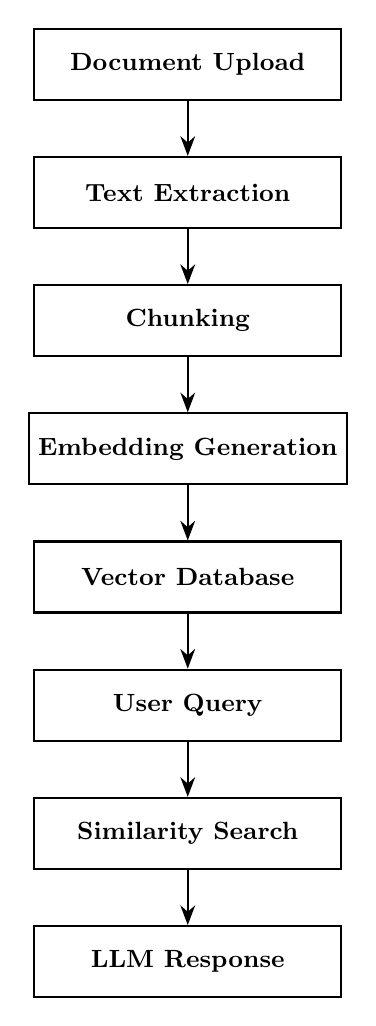
\begin{tikzpicture}[
    node distance=7mm,
    stage/.style={rectangle, draw=black, thick,
                  minimum width=3.9cm, minimum height=0.9cm,
                  align=center, font=\small\bfseries},
    arr/.style={-{Stealth[length=2.5mm]}, thick, draw=black}
]
    \node[stage] (upload) {Document Upload};
    \node[stage, below=of upload] (extract) {Text Extraction};
    \node[stage, below=of extract] (chunk) {Chunking};
    \node[stage, below=of chunk] (embed) {Embedding Generation};
    \node[stage, below=of embed] (vecdb) {Vector Database};
    \node[stage, below=of vecdb] (query) {User Query};
    \node[stage, below=of query] (sim) {Similarity Search};
    \node[stage, below=of sim] (llm) {LLM Response};

    \foreach \a/\b in {upload/extract, extract/chunk, chunk/embed, embed/vecdb, vecdb/query, query/sim, sim/llm}
        \draw[arr] (\a) -- (\b);
\end{tikzpicture}
\caption{Retrieval-Augmented Generation (RAG) pipeline used for document intelligence}
\label{fig:rag}
\end{figure}

\subsection{Pipeline Description}

When a document is uploaded, its text is first extracted from formats such as PDF, DOCX or plain text. The extracted text is then split into smaller, semantically coherent chunks, since embedding an entire document at once would lose the fine-grained context needed for accurate retrieval. Each chunk is passed through a pre-trained embedding model to produce a vector representation of its meaning, and these vectors are stored in a vector database for efficient similarity search.

When a user submits a query, either as a search term or a natural-language question, the same embedding model converts it into a vector, which is compared against the stored document vectors to find the most relevant chunks. For search, these chunks are returned directly. For question answering, the retrieved chunks are passed as context to a language model, which generates an answer grounded in the user's own documents rather than in the model's unrelated general knowledge. This keeps answers traceable back to the source material and reduces the risk of the model inventing information that is not actually present in the documents.

\section{Scalability Design}

NimbusVault's architecture is designed with horizontal scalability in mind, rather than treating it as an afterthought.

Storing file content in AWS S3 separately from metadata in PostgreSQL means each layer can be scaled according to its own load pattern; a spike in file uploads, for example, does not directly affect database load. Pre-signed URLs let file transfer bypass the application backend entirely, so the backend is not a bottleneck for large or frequent transfers. The backend itself is stateless, meaning it does not store session data locally, which allows multiple backend instances to run behind a load balancer without any need for session affinity. Deployment on AWS EC2, or an equivalent managed compute service, with auto-scaling allows capacity to adjust automatically as demand changes. Finally, computationally expensive tasks such as text extraction, chunking and embedding generation are handled by background workers coordinated through a message queue, so these tasks do not block or slow down the main API.

\section{Security Design}

Security is addressed at several layers of the platform. All authenticated requests require a valid, signed JWT, checked on every API call, and passwords are never stored in plain text; they are hashed using a strong, salted algorithm such as bcrypt before being saved. On the cloud side, AWS IAM policies restrict the application's permissions on S3 to the minimum required for it to function, and pre-signed URLs are both time-limited and scoped to a specific object and operation, so they cannot be reused indefinitely or for unrelated files. All communication between client and server is encrypted using HTTPS. Shared resources are protected by role-based access control, with owner, editor and viewer roles determining what actions a given user can perform, and sharing links use randomly generated tokens with configurable expiry to limit how long shared content remains accessible.

\section{Development Methodology}

The project will be developed in four phases, each building on the previous one to progressively add core, collaborative, operational and intelligent capabilities.

\begin{table}[h!]
\centering
\begin{tabular}{@{}>{\bfseries}p{2.6cm}p{4.4cm}p{6cm}@{}}
\toprule
\textbf{Phase} & \textbf{Focus Area} & \textbf{Key Deliverables} \\
\midrule
Phase 1 & MVP Cloud Storage & Authentication, upload/download, folder management, basic search \\
\midrule
Phase 2 & Security \& Collaboration & Secure sharing links, role-based access control, expiring permissions \\
\midrule
Phase 3 & Cloud Deployment \& DevOps & Containerisation, CI/CD pipeline, cloud deployment, monitoring \\
\midrule
Phase 4 & AI Document Intelligence & Text extraction, embeddings, vector database, RAG-based Q\&A \\
\bottomrule
\end{tabular}
\caption{Phase-wise development methodology}
\label{tab:phases}
\end{table}

\section{Evaluation Criteria}

The completed system will be assessed against the following measurable criteria.

\begin{table}[h!]
\centering
\begin{tabular}{@{}>{\bfseries}p{4.6cm}p{8.4cm}@{}}
\toprule
\textbf{Metric} & \textbf{Description / Target} \\
\midrule
Upload/download success rate & Percentage of file transfers completed without error, targeting near-100\% reliability \\
\midrule
API response time & Average latency of core backend endpoints under typical load \\
\midrule
Search accuracy & Relevance of results returned for keyword and semantic search queries \\
\midrule
AI response relevance & Correctness and grounding of RAG-generated answers, checked against source documents \\
\midrule
System reliability & Uptime and error rate of the deployed platform during evaluation \\
\midrule
Security validation & Results of authentication, authorisation and access-control testing \\
\bottomrule
\end{tabular}
\caption{Evaluation metrics for the completed system}
\label{tab:eval}
\end{table}

\section{Future Enhancements}

A number of extensions fall outside the current scope but are worth pursuing in future iterations of the project:

\begin{itemize}[leftmargin=1.2cm, itemsep=4pt]
    \item Zero-knowledge encryption for end-to-end confidential file storage
    \item A native mobile application for iOS and Android
    \item Team workspaces with organisation-level administration
    \item More detailed usage and behavioural analytics
    \item Kubernetes-based deployment for better orchestration and resilience
    \item Multi-region storage replication for improved durability and lower latency
\end{itemize}

\section{Risks and Mitigation}

\begin{table}[h!]
\centering
\begin{tabular}{@{}>{\bfseries}p{4.6cm}p{8.4cm}@{}}
\toprule
\textbf{Risk} & \textbf{Mitigation Strategy} \\
\midrule
Large file handling & Direct browser-to-S3 upload via pre-signed URLs avoids routing large payloads through the backend \\
\midrule
Unauthorized access & Layered checks using JWT authentication, AWS IAM policies and explicit permission checks \\
\midrule
Incorrect AI-generated answers & RAG pipeline grounds responses in retrieved source documents, with citations back to the source content \\
\midrule
Scope creep & Phase-based development with clearly defined deliverables for each phase \\
\bottomrule
\end{tabular}
\caption{Identified risks and corresponding mitigation strategies}
\label{tab:risks}
\end{table}

\section{Conclusion}

NimbusVault brings together full-stack web development, cloud infrastructure and applied AI within a single project. The storage architecture, based on separating metadata from file storage and transferring files directly through pre-signed URLs, reflects a practical, workable approach to building a scalable system rather than a purely theoretical one. The security measures used, including JWT authentication, password hashing, IAM policies and role-based access control, are standard practices in production systems and are applied here at a scope appropriate for an academic project.

The RAG-based document intelligence feature is what distinguishes NimbusVault from a simple storage clone, and its inclusion is intended to demonstrate familiarity with applied AI techniques such as embeddings, vector search and retrieval-grounded question answering. The phased development plan set out in this proposal is intended to keep the project achievable within the available time while still covering each of the major components described above.

\end{document}
